\section{How did you figure out how to be a parent?}
Perhaps reflecting on my childhood family experiences helped me think about how I would parent.
My experiences with children included having younger siblings and nieces and nephews that I helped to care for.
I also babysat for other people's children.
John and I spoke about parenting and we both felt that we wanted to parent differently than our parents.
One of the items that concerned us was the lack of comfort that we had speaking with our parents about some important issues.
Another was the sense of connection I felt emotionally with my parents.
I wanted my children to know that they were loved and their care was my priority.
\begin{figure}
\centering
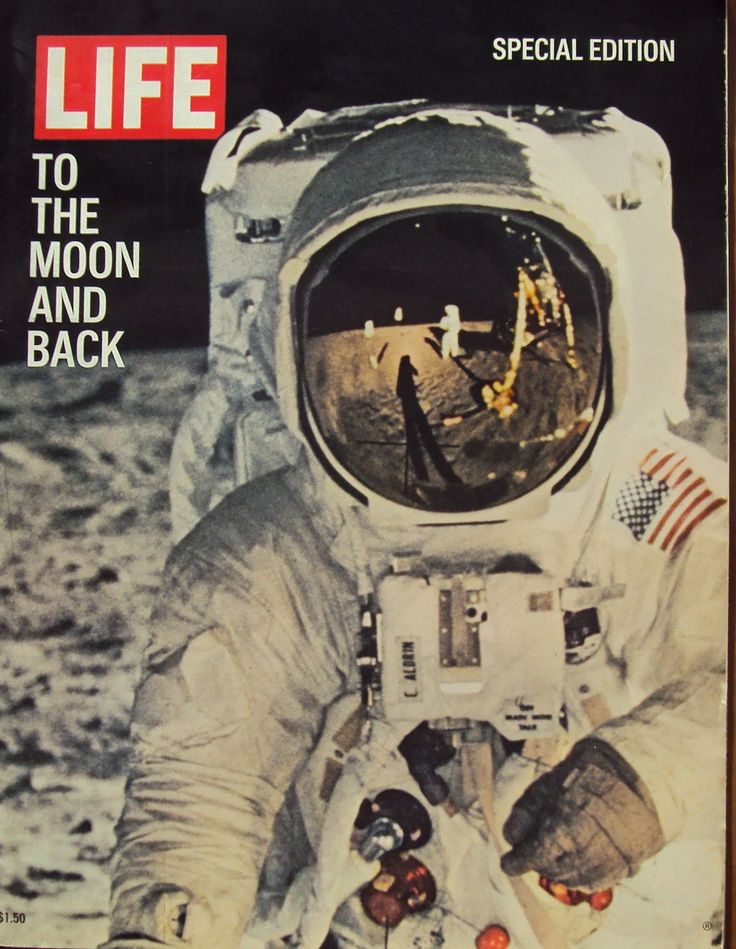
\includegraphics[width=0.9\textwidth]{our_family/2.jpg}
\caption{
The nursery was ready
}
\end{figure}

So was it enough to have these aspirations? We talked with other people about parenting and read books that we thought might be helpful.
One book was titled "Parenting for the Nineties".
We wanted to know what was being suggested in our culture at this time.
We found conflicting ideas and we made mistakes and changed course when we felt it was necessary.
One book we rejected was titled "God, the Rod and Your Child's Bod".

My brother Dan gave me advice that was helpful in understanding that I could not manage my children without managing myself.
"In any given situation you are the only one you can change," was a mantra that became important to me.
While it applied in many areas of living it affected who I became as a parent.
How could I help my children become compassionate adults who loved themselves and the people around them?
The image of journey became important to me as I thought about our life together as a family.
We each went through stages of growth and I realized that was also true for me as an adult.
One never stopped changing and learning.

I was also aware that we have only the current moment in which to live.
A question that was helpful was, "Will we be able to live with the decisions we have made."
I also know that my family learned that "When Mom is happy the family can be happy."
John and each of you children were willing to move with me to Indiana.
While not always easy, in the end, the move was life giving for me.

So how did I figure out how to parent? Perhaps by being present in the moment, listening and aware of what is being asked of me as a human being who loves and cares for those around me.

